\documentclass[10pt]{article}
\usepackage[a4paper,margin=2.2cm]{geometry}
\usepackage{fontspec}
\setmainfont{Charter}
\setsansfont{Helvetica Neue}
\newfontfamily\deva{Devanagari Sangam MN}[Scale=0.92]
\usepackage{microtype,booktabs,graphicx,xcolor,enumitem,amsmath,amssymb,caption}
\usepackage[numbers,sort]{natbib}
\usepackage[hidelinks]{hyperref}
\captionsetup{font=small,labelfont=bf}
\setlist{nosep,leftmargin=1.2em}
\definecolor{fail}{HTML}{B3261E}\definecolor{pass}{HTML}{1B7A3E}
\newcommand{\PASS}{\textcolor{pass}{\textbf{pass}}}\newcommand{\FAIL}{\textcolor{fail}{\textbf{fail}}}
\title{\vspace{-1.2em}\textbf{Missing Words: what one token's rows can hold in Gemma~4}}
\author{Sanjit Mathur\\\small SRM Institute of Science and Technology\\\small Draft of 26 November 2026. Code, frozen protocol and all raw outputs: [[repository link]]}
\date{\vspace{-1.5em}}
\begin{document}\maketitle

\begin{abstract}\noindent
Gemma~4 E2B and E4B give every token two learnt tables: an input embedding and a per-layer embedding (PLE) row that is read again in every decoder layer, and which accounts for about a third of E4B's parameters. We ask what a single token's rows can hold when every other weight is frozen, and we test the answers against rules fixed and hashed before the main runs. Training only the rows of one reserved token installs an arithmetic rule that carries over to unseen numbers and unseen question formats: 19 of 24 rules reach 80\% (mean 82.5\%, five seeds), whereas a random lookup table with no rule stays below 1\%. Neither table alone is enough (50\% and 58\% on eight rules), while the two together reach 92\%. The same mechanism repairs Hindi quantity words that both models misread, such as {\deva पौने} (``a quarter less than''), with outputs on text without the word left bit-identical; however LoRA remains more accurate, and two of our three pre-registered repair claims failed. Replacing every PLE row by the mean row costs Indian-script text 28 (E4B) and 45 (E2B) percentage points more extra loss than English, so the table matters most outside English. Finally, 214 of the 219 tokens that Google repaired in E4B's tokenizer on 3 November still have untrained per-layer rows, and a per-layer statistic finds 288 further tokens that the model cannot repeat; pruning 474 BPE merges fixes all but one of the 361 failing tokens we list. We report each failed prediction next to the ones that held.
\end{abstract}

\section{Introduction}
A model that has been trained on a language can still fail on one of its everyday words. Gemma~4 E4B answers none of 43 plain questions containing {\deva पौने दो लाख} (Rs~1,75,000) correctly, although it computes the same amounts when they are written as arithmetic; in an Indian payments or voice setting such a failure turns into a wrong amount rather than a refusal. The question this raises is whether the missing piece is the skill or only the word, and, if it is the word, whether a word can be added to a deployed model without disturbing anything else it does.

Gemma~4's small models make the second half of that question unusually clean. Because each token owns a per-layer row that only that token reads, gradient updates restricted to one token's rows cannot change the model's output on any text where the token is absent, a guarantee that holds exactly rather than approximately and that no adapter on shared weights provides. That property makes a token a natural unit for small, local edits, but it also leaves two open problems: how much behaviour can be packed into rows that were designed to carry lexical identity, and what the per-layer table stores in the first place.

We study both with a protocol that was written, hashed and frozen before the main runs, with five gates fixed in advance and eleven dated amendments recorded as they happened (Appendix~\ref{app:protocol}). Our findings are the following.
\begin{itemize}
\item One token's rows can hold a \emph{rule} rather than a lookup: on held-out numbers and three question formats never used in training, 19 of 24 arithmetic rules reach the pre-set 80\% bar on E4B, while ruleless tables do not, and the rule needs both tables (Section~\ref{sec:programs}).
\item Training a word's rows repairs Hindi fraction words with exactly zero change elsewhere, transferring to romanised Hindi and other scripts given a word list, but it is less accurate than LoRA and fails our own pre-registered bar for unseen formats on E4B (Section~\ref{sec:repair}).
\item The per-layer table behaves like multilingual memory: removing its token-specific content hurts several Indian scripts far more than English, on parallel text and in both models (Section~\ref{sec:languages}).
\item Untrained per-layer rows remain on tokens that the November tokenizer fix addressed, and the same signal locates a few hundred further broken tokens, which merge pruning repairs (Section~\ref{sec:tokens}).
\end{itemize}

\section{Per-layer embeddings in Gemma 4}
In E2B and E4B each token $t$ has, besides its input embedding $e_t\in\mathbb{R}^{d}$, a per-layer row $u_t\in\mathbb{R}^{L\times 256}$, with $L=42$ layers in E4B. In layer $l$ the residual stream $h$ receives $\mathrm{RMSNorm}\bigl(W_l\,(u_{t,l}+P_l e_t)\odot \mathrm{gelu}(G_l h)\bigr)$, so the row acts as a token-specific gate on a small projection of the hidden state; in E4B the table holds 2.82\,B numbers, around 35\% of the model. Two properties matter here. Each slice has norm close to one (1.007$\pm$0.021 in a sample), and rows of never-used tokens look like Gaussian noise (kurtosis 2.97, against 3.3--4.2 for real tokens). Further, the last 18 layers of E4B reuse keys and values from earlier layers, so the per-layer rows of a \emph{prompt} token at layers 23--41 are never read; we confirmed that their trained change is exactly zero, and an E4B word therefore needs 5{,}888 trainable numbers rather than 10{,}752 (layer 14 is the corresponding cut in E2B). Inference engines already skip these layers during prefill, so we make no claim about speed.

\paragraph{Editing one token.} Throughout, ``training a token'' means optimising only $e_t$ and $u_t$ for one reserved token while every other weight stays frozen, implemented with forward hooks on the official Hugging Face checkpoints in bfloat16. For words, a deterministic preprocessor maps the word (or a listed spelling of it) to the reserved token. Because no other token reads these rows, text without the token produces identical logits; we verify this on 85 unrelated prompts, where the largest change in any log-probability is $0.0$.

\section{One-token programs}\label{sec:programs}
\paragraph{Setup.} Each of 24 rules (for example $n+3$, $2n+1$, $n^2$, digit reversal, $n \bmod 10$) is installed into a fresh reserved token, written as ``\texttt{blick~$n$}''. Operands $11$--$99$ are split once into 59 training and 30 held-out values; training uses eight phrasings and 200 steps, and evaluation asks for held-out operands in three phrasings never used in training (a variable assignment, a JSON field and a word problem). Two controls replace the rule with a random permutation of the operands, which no rule can compress. We compare with the base model given the rule in words, a definition, or eight worked examples.

\begin{figure}[t]\centering
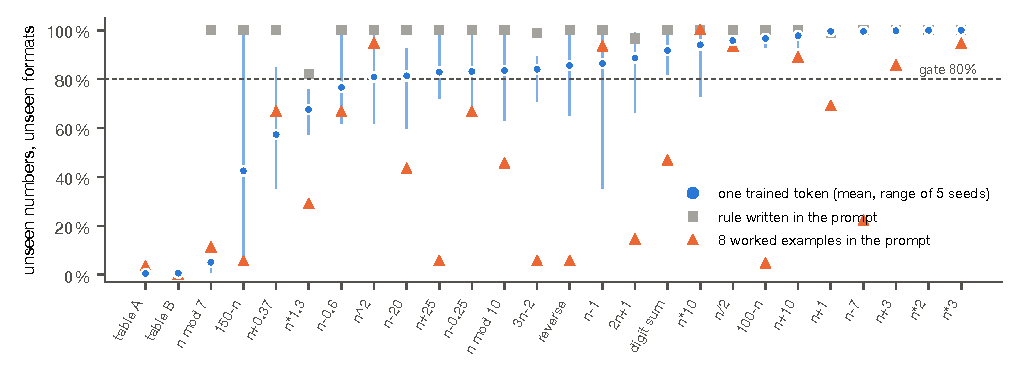
\includegraphics[width=\linewidth]{fig_programs.pdf}
\caption{\textbf{One token can hold a rule, not a table.} E4B, held-out operands in unseen formats, five seeds (dot: mean; line: range). Tables A and B are random permutations. Grey squares give the same rule written in the prompt, which remains the stronger way to obtain an answer; the point here is what the rows can store.}\label{fig:programs}
\end{figure}

\paragraph{Result.} Gate~1 required at least 16 of 24 rules at 80\% and both tables at most 5\%; it \PASS{}es with 19 of 24 rules (mean 82.5\%) and tables at 0.4\% and 0.7\% (Figure~\ref{fig:programs}). The failures are informative rather than random: $n \bmod 7$ (5\%) and $150-n$ (42\%) are not fitted even on training operands, which suggests that the rows can only point to computations that the frozen model already performs in one pass, whereas fractional offsets such as $+0.37$ (57\%) fit the training formats and fail to travel to the new ones. Two rules pass narrowly at 81\%, and the margin of the gate should be read accordingly. On E2B, eight rules with three seeds give a weaker partial replication, three of eight at 80\% and a mean of 80\%, with the ruleless table at 1.5\%.

\paragraph{Both tables are needed.} Training only the per-layer rows or only the input row (Figure~\ref{fig:tables}) reaches the training formats in almost every case but falls to a mean of 50\% and 58\% respectively in unseen formats, against 92\% for both. With only per-layer rows, most rules score zero in one of the three new formats, which points to the input row as the carrier of format-independent identity and the per-layer rows as the carrier of the operation. The single-table runs use three seeds and the joint runs five, and this analysis was added after the protocol was frozen (amendment A11).

\begin{figure}[t]\centering
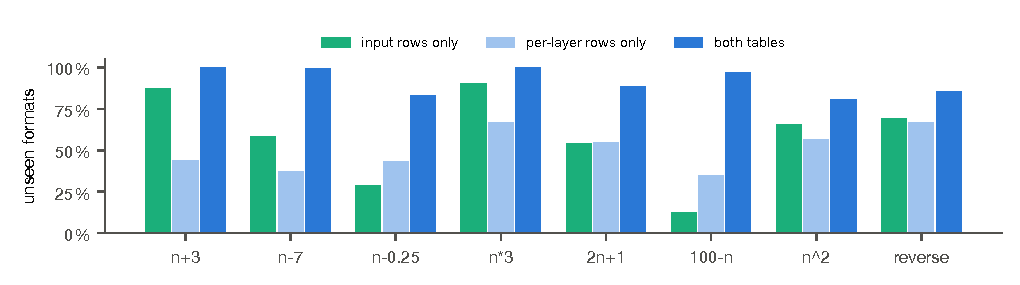
\includegraphics[width=\linewidth]{fig_tables.pdf}
\caption{\textbf{Neither table carries a rule alone.} E4B, unseen formats; single-table runs three seeds, both tables five seeds.}\label{fig:tables}
\end{figure}

\section{Repairing quantity words}\label{sec:repair}
\paragraph{Setup.} Five Hindi fraction words ({\deva सवा, साढ़े, पौने, डेढ़, ढाई}) are each given a token whose rows are trained for 160 steps on amounts built from them; the numbers 4, 7, 9, 11, 13, 16 and 19 are never used in training. We test four formats, three of them unseen, plus romanised Hindi and five other Indian languages, which share the words through a word list. Baselines are a glossary in the prompt, eight worked examples, input rows only, and LoRA (rank 8, query and value projections) with and without ``keep'' data covering other senses of the same words; LoRA is also given the same word list when crossing scripts, which the pilot had not done.

\begin{figure}[t]\centering
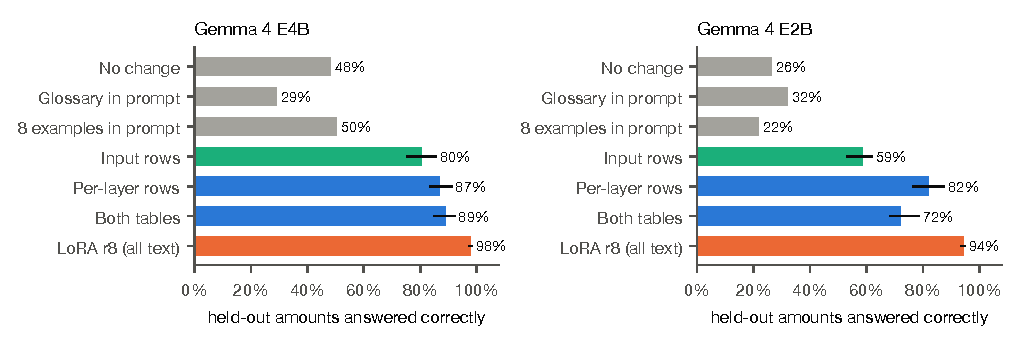
\includegraphics[width=\linewidth]{fig_repair.pdf}
\caption{\textbf{Word repair with all weights frozen.} Held-out amounts in four formats (288 items); lines mark the seed range. The row methods leave every output on unrelated text unchanged; LoRA changes 62 of 85 (E4B) and 69 of 85 (E2B).}\label{fig:repair}
\end{figure}

\paragraph{Result.} On E4B, per-layer rows raise accuracy from 48\% to 87\% (mean of five seeds), against 98\% for LoRA (Figure~\ref{fig:repair}); prompting with a glossary makes matters worse. Gate~2 asked for a doubling of the base score in each unseen format: E4B reaches 1.54$\times$, 1.43$\times$ and 1.97$\times$, so the gate \FAIL{}s, whereas E2B alone would pass (3.0$\times$, 3.0$\times$, 2.3$\times$). Gate~3 asked the rows to beat LoRA-with-the-word-list across scripts by ten points; they lose (E4B 77\% against 95\%, E2B 56\% against 80\%), so it also \FAIL{}s. Gate~4, that per-layer rows beat input rows in both models, \PASS{}es: $+6.4$ points on E4B (95\% interval 1.2 to 11.5) and $+23.3$ on E2B (15.5 to 31.4), bootstrapping over seeds and items. The honest summary is that the patch trades about ten points of accuracy for exact locality and a size of a few thousand numbers per word. Two costs remain: rows trained on E2B reduce correct readings of idioms that contain the same words from 60\% to 37\%, and ``keep'' data restores weight and time readings of the same words (to 100\% and 78\% on E4B) but not the idioms.

\section{What the per-layer table stores}\label{sec:languages}
We replace every token's per-layer rows by the mean row (and, as checks, by shuffled rows and by zeros) and measure the extra loss on 60 parallel Belebele passages in 24 languages. Gate~5 required the cost for nine Indian-script languages to exceed both English and six other Latin-script languages, with bootstrap intervals over passages excluding zero, in both models; it \PASS{}es (Figure~\ref{fig:languages}). Relative to English, Indian scripts lose 27.7 points more on E4B (24.5 to 30.9) and 45.1 more on E2B (40.6 to 49.7); relative to other Latin-script languages the differences are 11.0 (8.5 to 13.3) and 28.2 (25.6 to 30.8). The pattern is not uniform: Hindi and Bengali sit close to English, Thai and Tamil are high, and Kannada and Malayalam show the largest costs on both models. Ablating a table after training is not the same as training without it, but the result sits in tension with EmbeddingGemma~2, which drops a lookup table and improves on English-centred benchmarks, and it suggests that such a choice should be checked language by language.

\begin{figure}[t]\centering
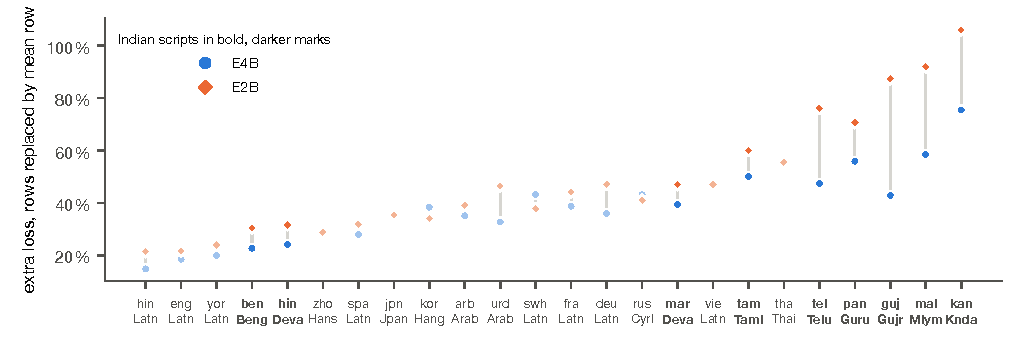
\includegraphics[width=\linewidth]{fig_languages.pdf}
\caption{\textbf{Per-layer rows matter most for several Indian scripts.} Extra loss per passage when every per-layer row is replaced by the mean row, as a share of the original loss; 60 parallel passages per language.}\label{fig:languages}
\end{figure}

\section{Broken tokens after the tokenizer fix}\label{sec:tokens}
On 3 November Google merged a change that makes 219 E4B tokens with collapsed input embeddings unreachable by the tokenizer. We find that 214 of them also have per-layer rows indistinguishable from never-trained ones, and that the same test across the vocabulary is useful. Tokens whose per-layer kurtosis falls below the 95th percentile of unused tokens fail a repeat test (``repeat this string exactly'') far more often than random tokens: 334 of 1{,}662 against 6 of 3{,}972 under the fixed tokenizer, which \PASS{}es the first claim of the token study. Removing the 434 merges that create them repairs 332 of the 334. A pre-registered claim that this per-layer statistic beats existing detectors \FAIL{}s: the under-trained-token method of Land and Bartolo finds more failing tokens in the top 500, and input-embedding kurtosis does slightly better in the top 400. We therefore report a union list. It contains 361 failing tokens, of which 288 produce unrelated output rather than a near-copy or the right sound in another script; pruning 474 merges fixes all but one. E2B has 489 truly broken tokens under the same rule. For an earlier 391-token list, pruning changed 14 of 2.69 million tokens of sample text, all Bengali or Tamil, but split 29 healthy compounds. A label-free alternative trains the broken tokens' rows against the model's own predictions on the pruned spelling, which recovers a held-out code prompt (12.5\% to 93\%, against 94.5\% for pruning) but not spelling tasks (14\% against 61\%), so pruning remains the better repair where it costs nothing.

\section{Predictions that failed}
Besides gates 2 and 3 and the detector claim, the pilot's ``translations work, reflections do not'' law was wrong once enough training operands were used ($100-n$ reaches 97\%); single per-layer neurons were not readable; random subspaces of up to 64 dimensions of a row learnt nothing; a dictionary sentence written by E4B itself was too weak a teacher for label-free word repair (11--13\%); and composing a fraction word with number words failed in one design (26\% to 26\%) and helped in a second, exploratory one (26\% to 53\%). Every one of these is in the released logs.

\section{Related work}
Neologism learning on Gemma~3 trains a single new input embedding to express behaviours and concepts \citep{hewitt}; we extend the idea to the per-layer table, to rules tested on unseen operands and formats, and to exact-locality checks. Row edits in n-gram memories and writability studies \citep{engram,writability} report little transfer to new question forms in smaller models, which our format results speak to directly. Function vectors \citep{fv}, numerical representations \citep{helix} and the inner lexicon of multi-token words \citep{lexicon} offer mechanisms that the rows might point to. Under-trained token detection \citep{magikarp} and retokenisation \citep{glitchpatch} precede our token study; GlitchPatch already reports a high rate of faulty tokens in Gemma~4 E4B under a broader definition, so our contribution there is the per-layer signal and the measured cost of pruning. Our parallel data are from Belebele \citep{belebele} and our main baseline is LoRA \citep{lora}.

\section{Limitations and next steps}
Results cover two small models, one family of arithmetic rules, one family of quantity prompts and five seeds at most; the E2B programs use three seeds and eight rules, and every Hindi test item has so far been checked by one native speaker. Bootstrap intervals for gate~4 were computed with a script written after the data had been seen, and two analyses (the single-table study and the classification of broken tokens) were added by amendment. The ablation removes a table after training and cannot say what a model trained without it would learn. The next steps are a speech-to-amount benchmark in seven Indian languages, a test of whether separately trained word patches merge without interference, and a 12B comparison, where the model has no per-layer table.

\paragraph{Note on assistance.} [[Owner to decide wording: e.g. ``Code and drafting were assisted by an AI coding assistant; the author designed and checked the study and is responsible for every claim.'']]

{\small
\begin{thebibliography}{9}\setlength{\itemsep}{1pt}
\bibitem[Hewitt et al.(2025)]{hewitt} J.~Hewitt, O.~Tafjord, R.~Geirhos, B.~Kim. Neologism learning. arXiv:2510.08506, ICLR 2026.
\bibitem[Engram(2026)]{engram} User as Engram. arXiv:2606.19172.
\bibitem[Writability(2026)]{writability} Writability of n-gram memories. arXiv:2610.21553.
\bibitem[Todd et al.(2024)]{fv} E.~Todd et al. Function vectors in large language models. arXiv:2310.15213.
\bibitem[Kantamneni and Tegmark(2025)]{helix} S.~Kantamneni, M.~Tegmark. Language models use trigonometry to do addition. arXiv:2502.00873.
\bibitem[Kaplan et al.(2024)]{lexicon} G.~Kaplan et al. From tokens to words: on the inner lexicon of LLMs. arXiv:2410.05864.
\bibitem[Land and Bartolo(2024)]{magikarp} S.~Land, M.~Bartolo. Fishing for Magikarp: automatically detecting under-trained tokens. arXiv:2405.05417.
\bibitem[GlitchPatch(2026)]{glitchpatch} GlitchPatch. arXiv:2610.04399.
\bibitem[Bandarkar et al.(2024)]{belebele} L.~Bandarkar et al. The Belebele benchmark. arXiv:2308.16884.
\bibitem[Hu et al.(2022)]{lora} E.~Hu et al. LoRA: low-rank adaptation of large language models. arXiv:2106.09685.
\end{thebibliography}}

\appendix
\section{Protocol and gates}\label{app:protocol}
{\small\begin{tabular}{@{}p{7.4cm}lp{5cm}@{}}\toprule
Gate (fixed before the main runs) & Outcome & Numbers\\\midrule
1 Programs: $\ge$16/24 rules at 80\%, tables $\le$5\% (E4B) & \PASS & 19/24; tables 0.4\%, 0.7\%\\
2 Repair: $\ge$2$\times$ base in all three unseen formats, zero drift & \FAIL & E4B 1.54/1.43/1.97$\times$; drift 0\\
3 Cross-script: rows beat LoRA + word list by $\ge$10 pts & \FAIL & E4B 77 vs 95; E2B 56 vs 80\\
4 Per-layer rows beat input rows, both models & \PASS & +6.4 [1.2, 11.5]; +23.3 [15.5, 31.4]\\
5 Mean-row cost: Indian $>$ English and $>$ other Latin, both models & \PASS & +27.7/+11.0 (E4B); +45.1/+28.2 (E2B)\\\bottomrule
\end{tabular}}

\smallskip\noindent Hardware: Colab L4 for E4B and most E2B runs; part of E2B repair on a T4 with the same frozen code. Total compute about 26 Colab units. The protocol file lists all amendments with times, including a paused and byte-verified resumption of the final runs.
\end{document}
